\documentclass{article}
\usepackage{fullpage,amsmath,amsthm,graphicx,enumitem}
\usepackage{multicol}
\usepackage{booktabs}
\usepackage{hyperref}
\usepackage{tikz}

\theoremstyle{definition}
\newtheorem{thm}{Theorem}
\newtheorem{question}[thm]{Question}
\newenvironment{solution}{\noindent\textit{Solution:}}{}

\title{ASEN 5264 Decision Making under Uncertainty\\
       Homework 1: Probabilistic Models}

\begin{document}

\maketitle

\section{Questions}

\begin{question} (15 pts)
    Consider the following joint distribution of three binary-valued random variables, \mbox{$A$, $B$, and $C$}:

    \begin{minipage}{0.3\linewidth}
        \vspace{1em}
    {\small
    \begin{tabular}{cccc}
        \toprule
            $A$ & $B$ & $C$ & $P(A,B,C)$ \\
        \midrule
            $0$ & $0$ & $1$ & $0.15$ \\
            $0$ & $1$ & $0$ & $0.05$ \\
            $0$ & $1$ & $1$ & $0.01$ \\
            $1$ & $0$ & $0$ & $0.14$ \\
            $1$ & $0$ & $1$ & $0.18$ \\
            $1$ & $1$ & $0$ & $0.29$ \\
            $1$ & $1$ & $1$ & $0.06$ \\
        \bottomrule
    \end{tabular}
    }
    \end{minipage}
    \begin{minipage}{0.7\linewidth}
        \begin{enumerate}[label=\alph*)]
            \item What is the probability of the outcome $A=0$, $B=0$, $C=0$?
            \item What is the marginal distribution of $A$?
            \item What is the conditional distribution of $A$ given $B=0$ and $C=1$?
        \end{enumerate}
    \end{minipage}
\end{question}

% \begin{question} (20 pts)
%     Let $B$ be a uniformly-distributed binary random variable and let $A$ be a real-valued random variable with the following conditional distribution:
%     $$A \mid B=0 \quad \sim \quad \mathcal{U}(0,2)$$
%     $$A \mid B=1 \quad \sim \quad \mathcal{U}(1,3)$$
%     \begin{enumerate}[nosep,label=(\alph*)]
%         \item Plot or draw the probability density functions for the conditional distribution of $A$.
%         \item Plot or draw the marginal density function of $A$.
%         \item What is the probability that $A=1.5$?
%         \item What is the probability that $A \in [1.5, 1.6]$?
%     \end{enumerate}
% \end{question}

\begin{question} (20 pts)
    2\% of women at age forty who participate in routine screening have breast cancer. 86\% of those with breast cancer will get positive mammograms. 8\% of those without breast cancer will also get positive mammograms. A woman in this age group had a positive mammogram in a routine screening. What is the probability that she actually has breast cancer?
\end{question}

\begin{question} (20 pts) Suppose that $A$, $B$, and $C$ are binary random variables with $P(A=1) = 0.5$, $P(B=1|A=1) = 0.8$, $P(B=1|A=0) = 0.2$, $P(C=1|B=1) = 0.9$, $P(C=1|B=0) = 0.3$, and the following Bayesian network structure:
    \begin{center}
        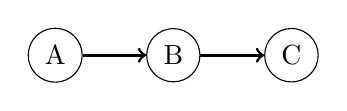
\begin{tikzpicture}
            \node[shape=circle,draw=black] (A) at (0,0) {A};
            \node[shape=circle,draw=black] (B) at (1.5,0) {B};
            \node[shape=circle,draw=black] (C) at (3,0) {C};
            \path [->,line width=1pt] (A) edge node[left]{}(B);
            \path [->,line width=1pt] (B) edge node[left]{}(C);
        \end{tikzpicture}
    \end{center}
If we observe that $C=1$, what is the probability that $B=1$?
\end{question}

\begin{question} (20 pts)
    Consider the following Bayesian network structure:

    \begin{center}
    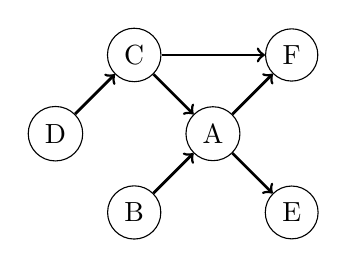
\begin{tikzpicture}
        \node[shape=circle,draw=black] (D) at (0,0) {D};
        \node[shape=circle,draw=black] (A) at (2,0) {A};
        \node[shape=circle,draw=black] (C) at (1,1) {C};
        \node[shape=circle,draw=black] (F) at (3,1) {F};
        \node[shape=circle,draw=black] (E) at (3,-1) {E};
        \node[shape=circle,draw=black] (B) at (1,-1) {B};
        \path [->,line width=1pt] (C) edge node[left]{}(A);
        \path [->,line width=1pt] (D) edge node[left]{}(C);
        \path [->,line width=1pt] (B) edge node[left]{}(A);
        \path [->,line width=1pt] (A) edge node[left]{}(E);
        \path [->,line width=1pt] (A) edge node[left]{}(F);
        \path [->,line width=1pt] (C) edge node[left]{}(F);
    \end{tikzpicture}
    \end{center}

    \begin{enumerate}[nosep,label=\alph*)]
        \item Is it possible to conclude from the structure that $B \perp F \mid C$? Justify your answer.
        \item Is it possible to conclude from the structure that $B \perp F \mid A$? Justify your answer.
        \item Is it possible to conclude from the structure that $B \perp E \mid A$? Justify your answer.
    \end{enumerate}
\end{question}

% \begin{question} (35 pts)
% Suppose that a stationary stochastic process $\{x_t\}$ is defined by the following equation: $x_{t+1} = 1.5 \, x_t - x_{t-1} + v_{t}$ where $v_t$ are independent, identically distributed random variables with $v_t \sim \mathcal{N}(\mu=0.0, \sigma^2=0.04)$.
%     \begin{enumerate}[nosep,label=(\alph*)]
%         \item Simulate and plot 10 20-step trajectories sampled from this process with $x_0 = x_{-1} = 1$ (You may use any programming language, but, as always, submit your code).
%         \item Is this process a Markov process if the state is defined as $x_t$? Why or why not?
%         \item If you did not have access to the equations defining the process and instead only had access to the trajectories you generated, what evidence could you use to convince someone that this process is or is not Markov?
%         \item What would you need to include in the state to create a Markov process that can be used to generate $\{x_t\}$? To answer this, define a new process $\{y_t\}$ that is Markov.
%     \end{enumerate}
% \end{question}

(assignment continues on next page)

\pagebreak

\section{Auto-graded Programming}

\begin{question} (20 pts autograder + 5 pts code)
    In this exercise, you will write and test a Julia function to ensure that you can get Julia and the course-specific code running and help you learn how to do a task that sometimes trips students up in homework 2. Your function should take two arguments:
    \begin{itemize}[nosep]
        \item \texttt{a}: a matrix, and
        \item \texttt{bs}: a non-empty vector of vectors.
    \end{itemize}
    The function should multiply all of the vectors in \texttt{bs} by \texttt{a} and then return a vector where the $i$th element is the maximum of the $i$th elements of all of the resulting vectors, that is, the \emph{elementwise} maximum of the resulting vectors.

    Example: if
    \begin{equation}
        \texttt{a} = \begin{bmatrix} 2 & 0 \\ 0 & 1 \end{bmatrix}  \text{ and } \texttt{bs} \text{ has the vectors } \begin{bmatrix} 1 \\ 2 \end{bmatrix} \text{ and } \begin{bmatrix} 2 \\ 1 \end{bmatrix},
    \end{equation}
    then, after multiplication, the resulting vectors are
    \begin{equation}
        \begin{bmatrix} 2 \\ 2 \end{bmatrix} \text{ and } \begin{bmatrix} 4 \\ 1 \end{bmatrix} \text{, and the elementwise maximum that should be returned is } \begin{bmatrix} 4 \\ 2 \end{bmatrix} \text{.}
    \end{equation}

    In order to get full-credit, the function must be completely ``type-stable'' (see the \href{https://docs.julialang.org/en/v1/manual/performance-tips/#Write-%22type-stable%22-functions}{``Performance Tips'' section of the Julia manual}). Your function should always return a vector with the same element type as \texttt{a}. You can assume the vectors in \texttt{bs} will have the same element type as \texttt{a}, but you should be able to handle \texttt{a} with any numeric element type.

    Evaluate this function with \texttt{DMUStudent.HW1.evaluate} and submit the resulting json file \textit{along with a listing of the code}. A score of 1 will receive full credit.
\end{question}

\end{document}
